\documentclass[12pt,a4paper]{article}
\usepackage{verbatim}
\usepackage{graphicx}
\usepackage{amsmath}
\usepackage{float}
\author{ZHANG Xiao Research Intern in IBM CRL}
\title{Network 20q HW6}

\begin{document}
\maketitle
\pagebreak

\section{Probability Distribution}
In this question, we need to compare the distribution of three distribution.

We could use the PDF of three functions to generate the graph.

The PDF of Pareto distribution is:
\begin{equation}
f(x) = \frac{\alpha*x_{m}^{\alpha}}{x^{\alpha+1}}  \quad  for \quad x \geq x_m
\end{equation}

The PDF of normal distribution is:
\begin{equation}
f(x) = \frac{e^-\frac{(x-\mu)^2}{2\sigma^2}}{\sqrt{2\pi\sigma^2}}
\end{equation}

The PDF of log-normal distribution is:
\begin{equation}
f(x) = \frac{e^-\frac{(ln x-\mu)^2}{2\sigma^2}}{x\sqrt{2\pi\sigma^2}}
\end{equation}

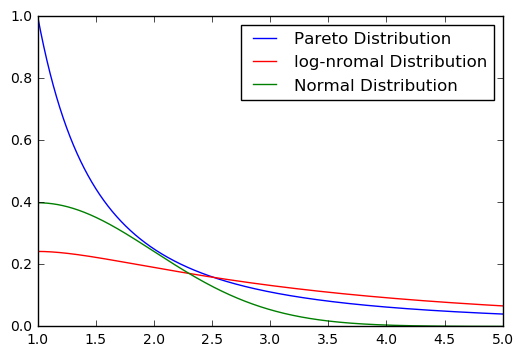
\includegraphics{PIC/distribution.png}

Then we could draw the log-log plot of the three distribution function:

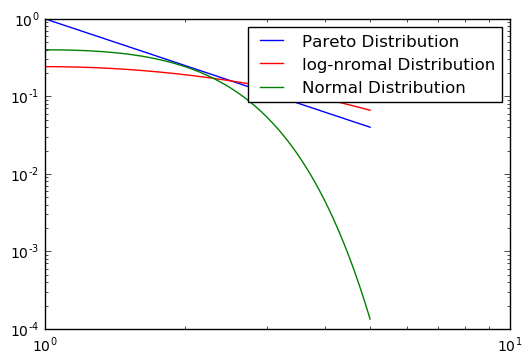
\includegraphics{PIC/distribution-log.png}

We could see that, the log-log plot of Pareto distribution is a straight line.
We could conclude that, log-normal distribution is more similar to Pareto distribution.

\section{$\alpha$ fairness utility function}

The $\alpha$ fairness utility function is:
\begin{equation}
U_{\alpha}(x) = \frac{x^{1-\alpha}}{1-\alpha} \quad (when \quad x \neq 1)
\end{equation}
\begin{equation}
U_{\alpha}(x) = \log{x} \quad (when \quad x \neq 1)
\end{equation}
\subsection{a}
Draw the function in the same graph:

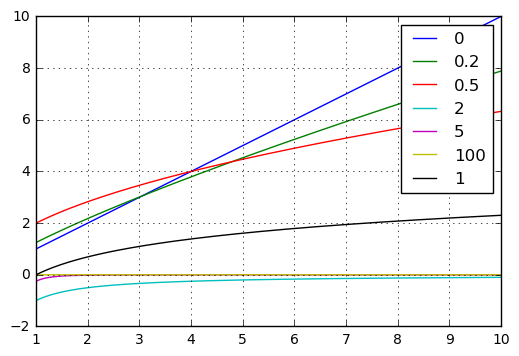
\includegraphics{PIC/fairness.png}

From the trend of various $\alpha$, we could conclude that, with the increase of $\alpha$, the seems decrease, which mean the function's change seems more steady. 

\subsection{b}
We already have the utility function:
\begin{equation}
U(x) = \arctan{x}
\end{equation}
Then we could have:
\begin{equation}
U'(D(p)) = \arctan{D(p)} = \frac{1}{1+D(P)^{2}} = p
\end{equation}
Then demand function would be:
\begin{equation}
D(p) = \sqrt{\frac{1}{p} - 1}
\end{equation}
The demand elasticity is:
\begin{equation}
-\frac{\partial D(p) / \partial p}{D(p)/p} = \frac{1}{2}*\frac{1}{\sqrt{\frac{1}{p}-1}} * (-1*\frac{1}{p^2}) =\frac{1}{2(1-p)}
\end{equation}
\subsection{c}
\begin{equation}
U_{\alpha}(x) = \frac{x^{1-\alpha}}{1-\alpha}
\end{equation}
And
\begin{equation}
U'_{\alpha}(x) = (\frac{x^{1-\alpha}}{1-\alpha})' = x^{-\alpha} = D(p)^{-\alpha} = p
\end{equation}
So
\begin{equation}
D(p)= p^{-\frac{1}{\alpha}}
\end{equation}
The demand elasticity is:
\begin{equation}
-\frac{\partial D(p) / \partial p}{D(p)/p} = \frac{1}{\alpha}*p^{-\frac{1}{\alpha}-1}*p*p^{\frac{1}{\alpha}} = \frac{1}{\alpha}
\end{equation}

\end{document}